 \chapter{Matplotlib: visualización gráfica}


\section{Una primera aproximación}

Una de las características de Matplotlib es la facilidad con la que se puede 
comenzar a trazar gráficas, vea el siguiente código:

\begin{python}
import matplotlib.pyplot as plt

plt.plot([5,10,6,-10,15,1])
plt.show()
\end{python}

El código anterior produce la gráfica mostrada en la figura \ref{fig:grafica_01a}. Como puede observar son solamente 
tres líneas de instrucciones, la primera sirve para importar el módulo \code{pyplot} de Matplotlib, el cual contiene 
muchas de las funciones útiles para el trazo de gráficas; la segunda línea ejecuta la función \code{plot} pasando como 
argumento una lista de valores numéricos, y finalmente la tercera línea se encarga de mostrar el elemento gráfico 
resultante en una ventana. 

Se puede obtener un resultado un poco más \textit{trabajado} con unas cuantas líneas más, tal como se 
muestra en la figura \ref{fig:grafica_01b}. Esta gráfica contiene un poco más de información, lo cual es 
deseable para cualquier representación de este tipo.

\begin{python}
import matplotlib.pyplot as plt

plt.plot([0,1,2,3,4,5], [5,10,6,-10,15,1], 'r--o', label="Partícula 1")
plt.xlabel("Tiempo (s)")
plt.ylabel("Posición (m)")
plt.title("Una primera aproximación")
plt.text(2,7,"$ P_1 (2,6) $", color="b")
plt.legend()
plt.grid(ls="--", color="#dadada")
plt.show()
\end{python}


\begin{figure}[h!]
\begin{subfigure}{0.48\textwidth}
\centering
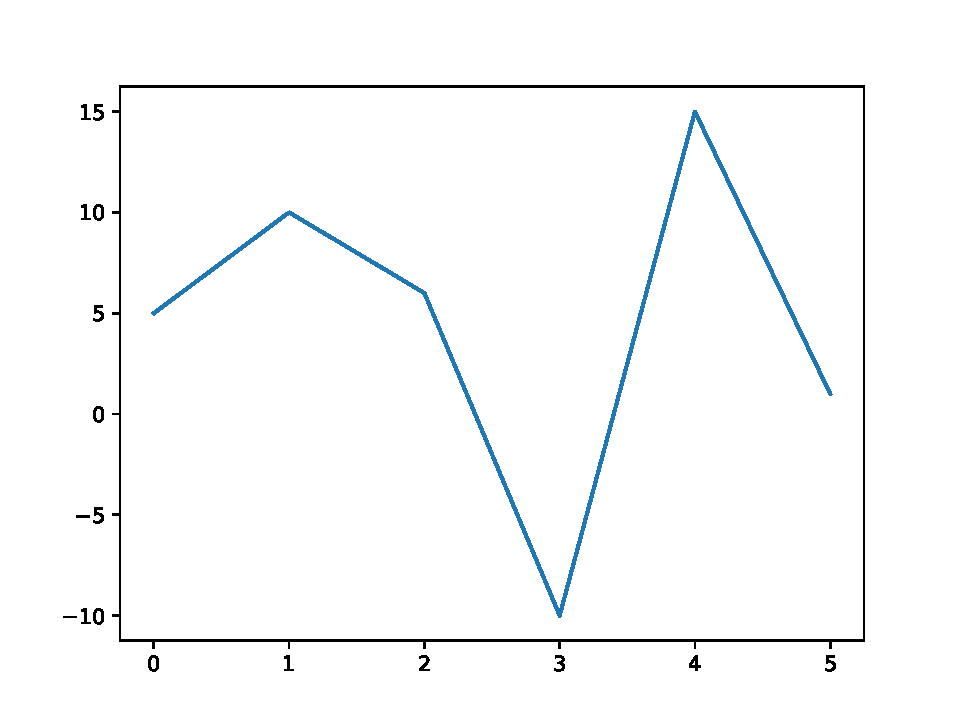
\includegraphics[width=0.9\textwidth]{img/ch03/grafica_01a.pdf}
\captionof{figure}{}
\label{fig:grafica_01a}
\end{subfigure}~
\begin{subfigure}{0.48\textwidth}
\centering
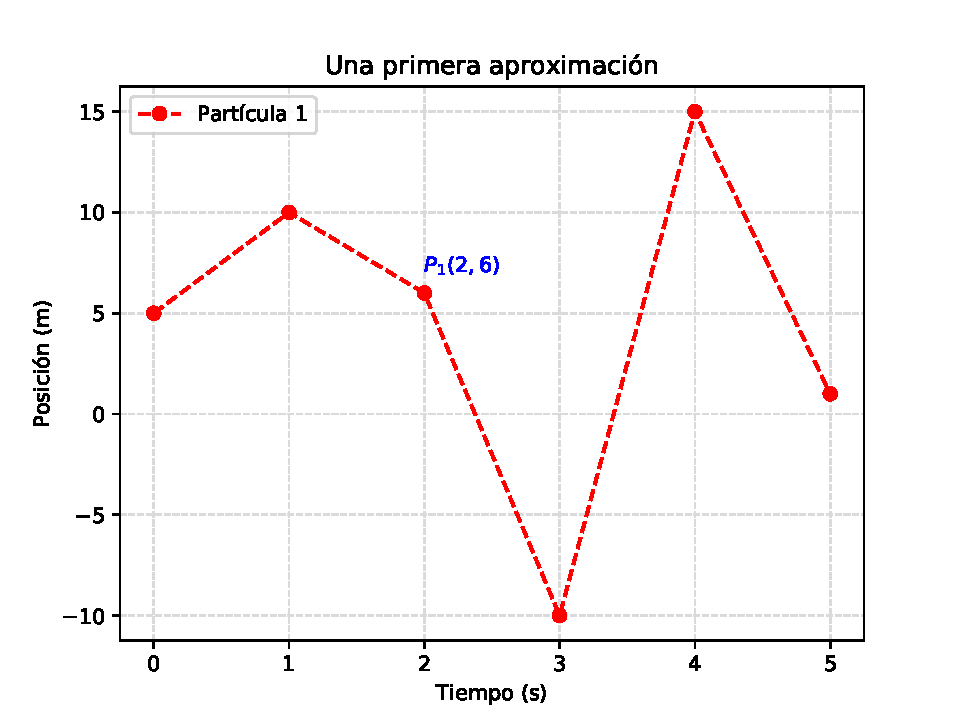
\includegraphics[width=0.9\textwidth]{img/ch03/grafica_01b.pdf}
\captionof{figure}{}
\label{fig:grafica_01b}
\end{subfigure}

\caption{}
\end{figure}



\section{La función \code{plot}}

La función \code{plot} está contenida en el módulo \code{pyplot} y básicamente con esta se produce cualquier gráfica 
bidimensional en coordenadas rectangulares. Esta función soporta varias maneras de ejecutarla dependiendo la cantidad 
de argumentos que se pasen. 

La forma más básica de la función \code{plot} es pasarle un sólo argumento, por ejemplo:

\begin{python}
import matplotlib.pyplot as plt

plt.plot([1,2,3,4,5])
plt.show()
\end{python}

Lo anterior produce una gráfica como la mostrada en la figura \ref{fig:plot_one_argument}. Al pasarle un sólo argumento, 
este se toma como los valores de la coordenada vertical, y se asume que la horizontal varía de 0 a N-1, donde N es el 
número de elementos contenidos en la lista de valores que se introducen.

\begin{figure}[h!]
\centering
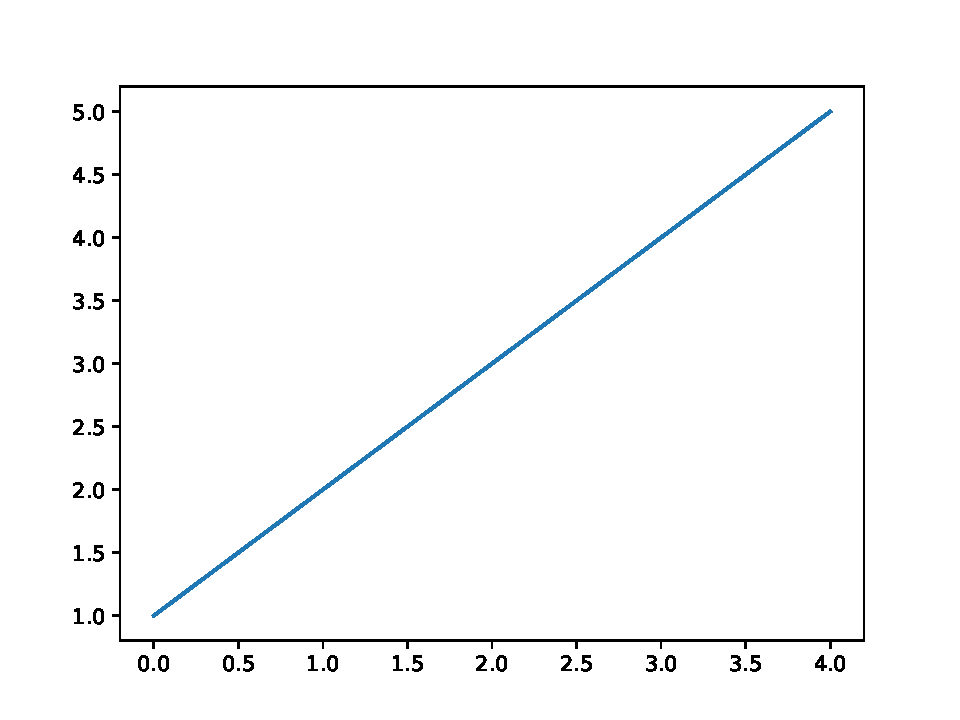
\includegraphics[width=0.55\textwidth]{img/ch03/plot_one_argument.pdf}
\captionof{figure}{}
\label{fig:plot_one_argument}
\end{figure}

La sintaxis más habitual es introducir dos argumentos, donde el primero contiene una lista \code{X} que define los valores 
de la coordenada horizontal, y el segundo una lista \code{Y} correspondiente a los valores de la coordenada vertical, 
por ejemplo:

\begin{python}
import matplotlib.pyplot as plt

plt.plot([10,25,30,60,70,100], [100,200,-100,300,0,-250])
plt.show()
\end{python}

En la figura \ref{fig:plot_two_argument} se muestra la gráfica resultante.

\begin{figure}[h!]
\centering
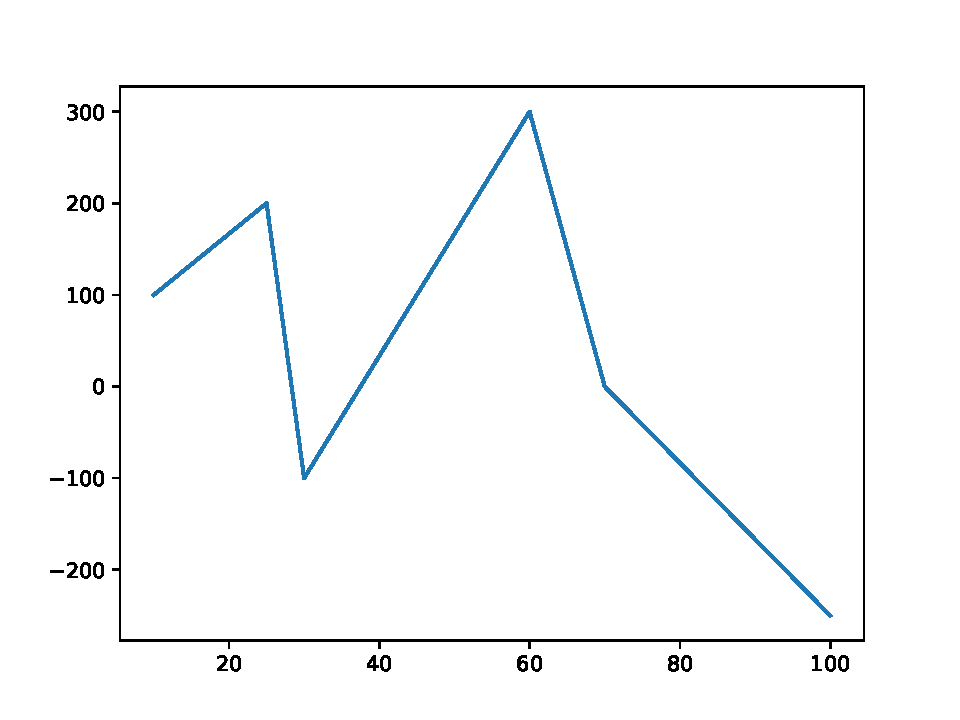
\includegraphics[width=0.55\textwidth]{img/ch03/plot_two_argument.pdf}
\captionof{figure}{}
\label{fig:plot_two_argument}
\end{figure}


\subsection{Graficando funciones matemáticas}

En matemáticas una función es una relación que asigna elementos de un conjunto de manera 
unívoca a otro conjunto. Usualmente una función matemática se puede representar 
mediante una gráfica en coordenadas cartesianas, colocando uno de los conjuntos en el 
eje horizontal y el otro en el vertical.

Utilizando Python, y de manera específica la librería NumPy, se pueden evaluar las funciones 
matemáticas en un intervalo determinado y en una cantidad finita de puntos. 
Por ejemplo, suponga que se requieren calcular todos los pares coordenados correspondientes 
a la función $ y = \cos x $ en el intervalo $ 0 \leq x \leq 5 $, en Python se tendría que definir 
como:

\begin{python}
import numpy as np

x = np.linspace(0,5)
y = np.cos(x)
\end{python}

Las variable \code{x} es un arreglo de NumPy que contiene 50 valores linealmente equiespaciados entre 
0 y 5, la variable \code{y} es también un arreglo de NumPy que resulta de aplicar la función coseno 
a cada valor de \code{x}.

De manera similar a lo anterior se procederá a definir y graficar la función 
$y = e^{-0.1x} \cos x $ en el intervalo $ 0 \leq x \leq 30 $:

\begin{python}
import matplotlib.pyplot as plt
import numpy as np

x = np.linspace(0, 30)
y = np.exp(-0.1*x)*np.cos(x)
plt.plot(x,y)
plt.show()
\end{python}

La gráfica resultante se muestra en la figura \ref{fig:plot_function}. La cantidad de puntos 
a evaluar es una cuestión muy importante, ya que de esto depende la correcta visualización del 
comportamiento de una función. Naturalmente, entre más puntos evaluados mejor será la apreciación 
que se tenga de la curva en cuestión, pero implica un mayor gasto de memoría para guardar y evaluar 
todos los datos. En las figuras \ref{fig:plot_function_more_points} y \ref{fig:plot_function_less_points} 
se muestra la misma función graficada en el mismo intervalo pero con 1000 y 5 puntos evaluados 
de manera respectiva, notará la diferencia entre los tres casos, es evidente que en el caso de los 
5 puntos \textit{se} pierde muchísima información.

\begin{figure}[h!]
\centering
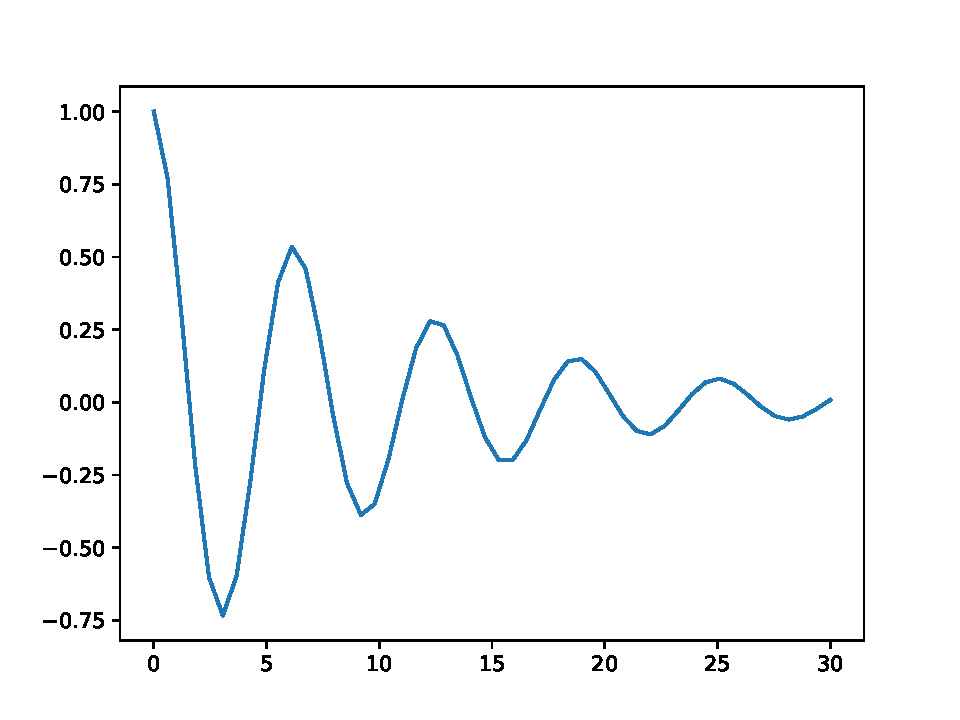
\includegraphics[width=0.55\textwidth]{img/ch03/plot_function.pdf}
\captionof{figure}{}
\label{fig:plot_function}
\end{figure}

\begin{figure}[h!]
\begin{subfigure}{0.48\textwidth}
\centering
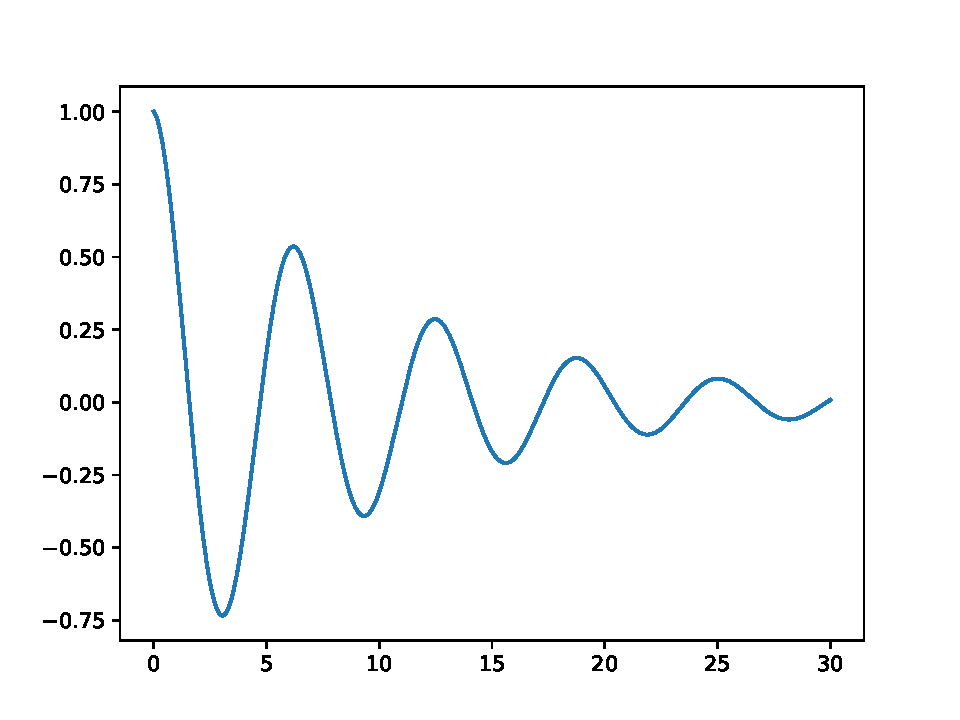
\includegraphics[width=0.9\textwidth]{img/ch03/plot_function_more_points.pdf}
\captionof{figure}{}
\label{fig:plot_function_more_points}
\end{subfigure}~
\begin{subfigure}{0.48\textwidth}
\centering
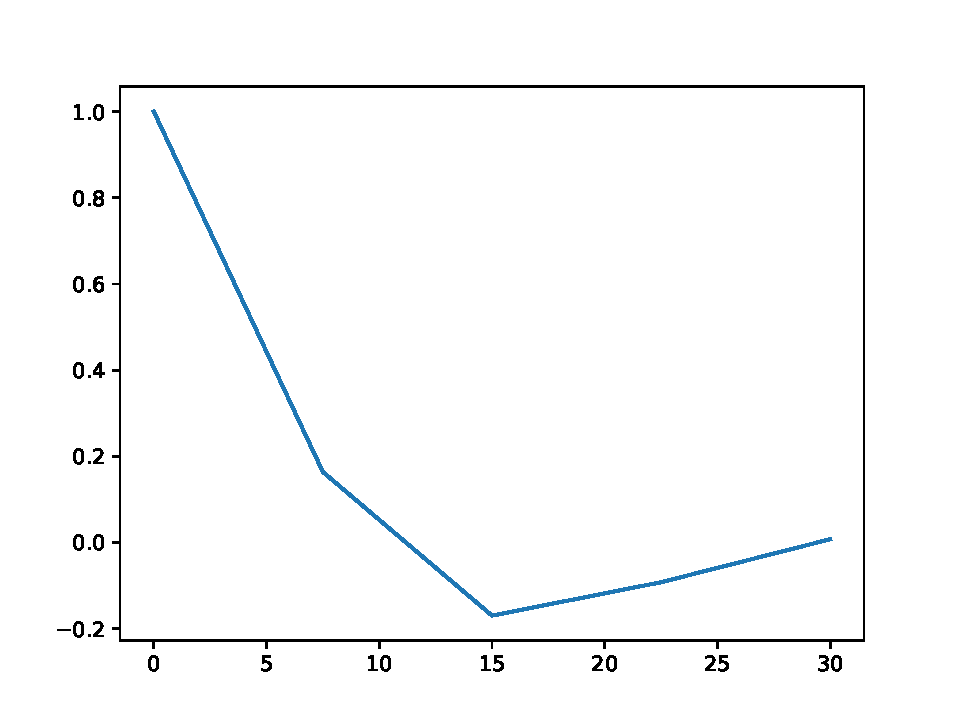
\includegraphics[width=0.9\textwidth]{img/ch03/plot_function_less_points.pdf}
\captionof{figure}{}
\label{fig:plot_function_less_points}
\end{subfigure}

\caption{}
\end{figure}


\subsection{Modificando el color, estilo y grosor de línea}

La función \code{plot} acepta argumentos adicionales que sirven para modificar y controlar características de 
la línea que se grafica. 

Se puede pasar un tercer argumento que contenga una combinación de color y estilo de línea. Por ejemplo:

\begin{python}
import matplotlib.pyplot as plt
import numpy as np

x = np.linspace(0, 30)
y = np.exp(-0.1*x)*np.cos(x)
plt.plot(x, y, "r--")
plt.show()
\end{python}

El código anterior genera una gráfica con una línea en color rojo (\code{r}) y un estilo de línea discontinua 
(\code{-{}-}), tal como se muestra en la figura \ref{fig:plot_color_and_style}. Si en lugar 
del string \code{'r-{}-'} se coloca \code{'go'}, se obtiene una gráfica como la mostrada en la 
figura \ref{fig:plot_color_and_style_02}, podrá inferir que \code{g} refiere al color 
verde (green) y \code{o} justamente al uso de esta como símbolo para representar cada punto.

\begin{figure}[h!]
\begin{subfigure}{0.48\textwidth}
\centering
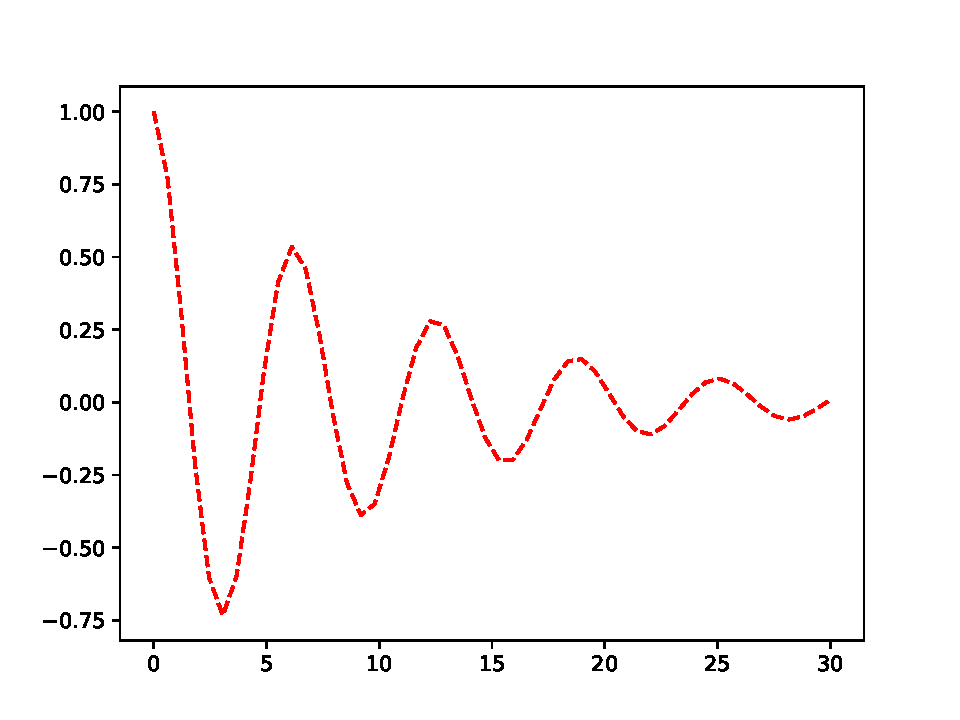
\includegraphics[width=0.9\textwidth]{img/ch03/plot_color_and_style.pdf}
\captionof{figure}{}
\label{fig:plot_color_and_style}
\end{subfigure}~
\begin{subfigure}{0.48\textwidth}
\centering
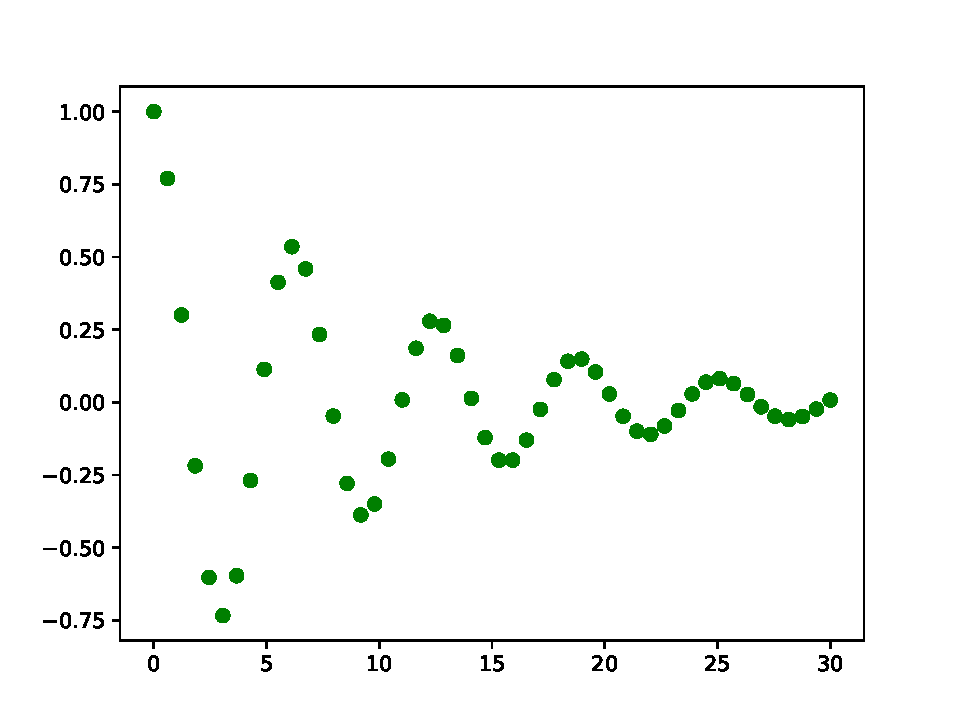
\includegraphics[width=0.9\textwidth]{img/ch03/plot_color_and_style_02.pdf}
\captionof{figure}{}
\label{fig:plot_color_and_style_02}
\end{subfigure}

\caption{}
\end{figure}


En \link{https://matplotlib.org/api/markers_api.html} se muestra una tabla con los símbolos (markers) 
disponibles para utilizar en la función \code{plot}. En \link{https://matplotlib.org/api/colors_api.html} 
puede consultar información respecto a los colores que puede abreviar mediante un sólo caracter.

Además de la forma anterior, también es posible especificar el color y estilo de línea utilizando 
\textit{keyword arguments}, obtendrá el mismo resultado que en la figura \ref{fig:plot_color_and_style} si 
utiliza el siguiente código:

\begin{python}
import matplotlib.pyplot as plt
import numpy as np

x = np.linspace(0, 30)
y = np.exp(-0.1*x)*np.cos(x)
plt.plot(x, y, linestyle="--", color="r")
plt.show()
\end{python}

En ambos casos se especifica un cierto estilo de línea y color, con la diferencia 
notoria de la sintaxis. 

Utilizar \textit{keyword arguments} es una manera más general, puesto que la definición con strings 
no funciona para los casos en que se requieren colores que no se pueden especificar con 
un sólo caracter, por ejemplo, Matplotlib dispone de un color llamado \code{coral} y 
este no puede ser invocado mediante un sólo caracter, hace falta escribir todo el nombre.

El siguiente código produce la gráfica mostrada en la figura \ref{fig:plot_color_and_style_03}, 
note que la clave \code{marker} define el símbolo utilizado para representar cada punto. 

\begin{python}
import matplotlib.pyplot as plt
import numpy as np

x = np.linspace(0, 30)
y = np.exp(-0.1*x)*np.cos(x)
plt.plot(x, y, linestyle="-", color="coral", marker="*")
plt.show()
\end{python}

En la figura \ref{fig:plot_color_and_style_04} se muestra una gráfica bastante similar, 
únicamente difieren en el grosor de la línea, mismo que es controlado con la clave 
\code{linewidth}, del código anterior sólo habría que agregar el argumento \code{linewidth} 
a la función \code{plot}.

\begin{python}
plt.plot(x, y, linestyle="-", color="coral", marker="*", linewidth=3)
\end{python}


\begin{figure}[h!]
\begin{subfigure}{0.48\textwidth}
\centering
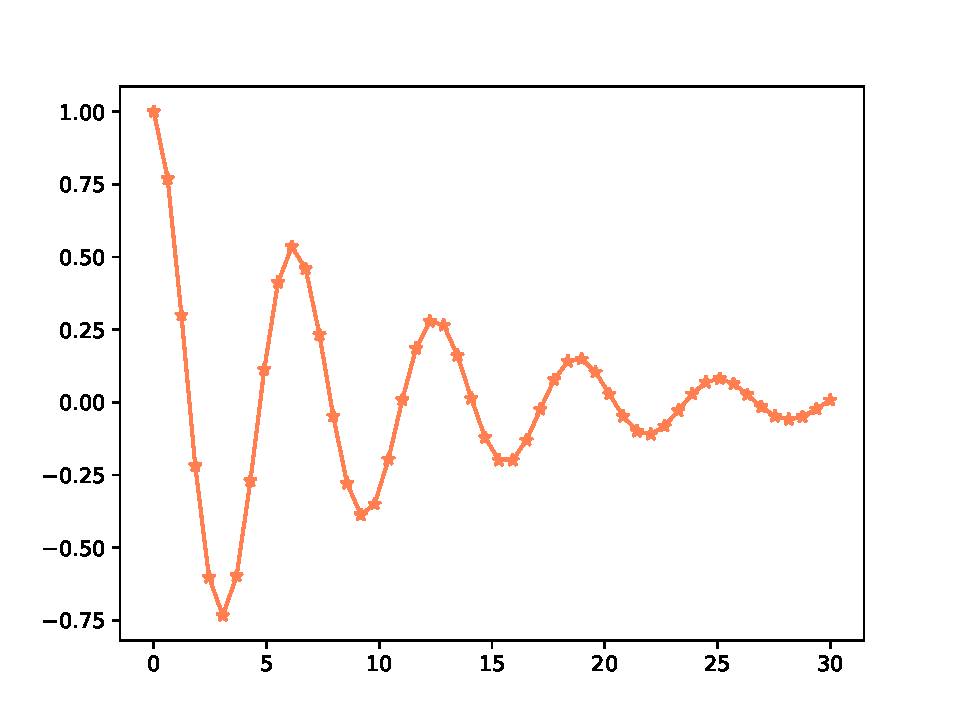
\includegraphics[width=0.99\textwidth]{img/ch03/plot_color_and_style_03.pdf}
\captionof{figure}{}
\label{fig:plot_color_and_style_03}
\end{subfigure}~
\begin{subfigure}{0.48\textwidth}
\centering
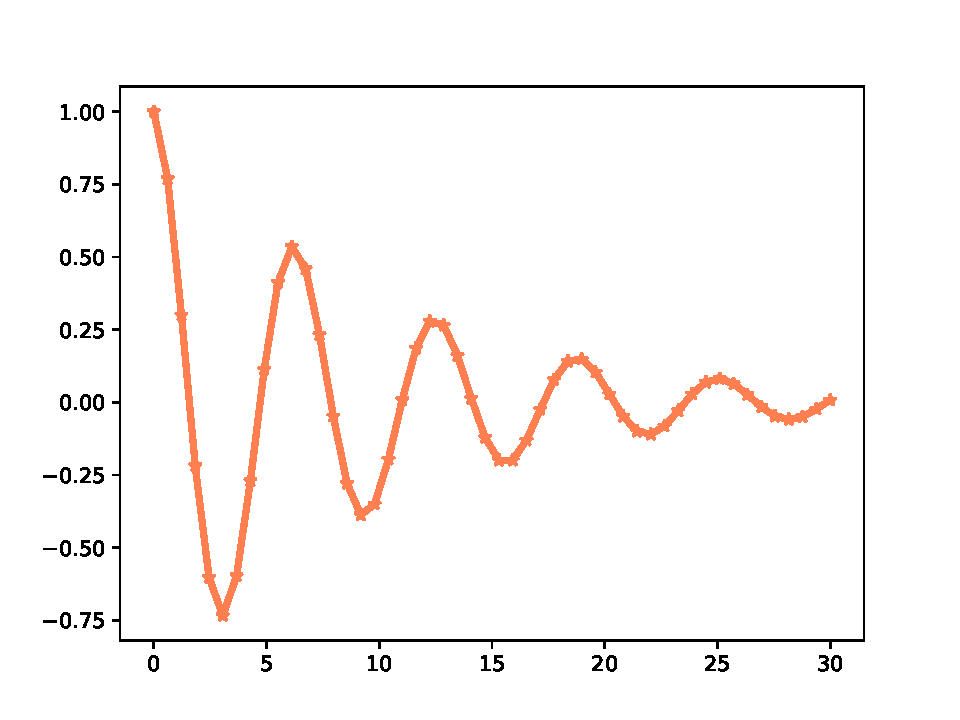
\includegraphics[width=0.99\textwidth]{img/ch03/plot_color_and_style_04.pdf}
\captionof{figure}{}
\label{fig:plot_color_and_style_04}
\end{subfigure}

\caption{}
\end{figure}

\subsection{Título de gráfica, etiquetas de ejes y nombres de curvas}

Por su naturaleza las gráficas nos sirven para presentar y/o visualizar información de ciertos datos, para 
lo cual se hace necesario especificar información descriptiva de lo que se muestra. Es muy común 
que se agreguen etiquetas a los ejes horizontal y vertical, así como el nombre de gráfica. Además, si 
se está graficando más de una curva, se hace necesario especificar a que refiere cada una de ellas.

El siguiente código produce la gráfica mostrada en la figura \ref{fig:plot_xlabel_ylabel_title}. 

\begin{python}
import matplotlib.pyplot as plt
import numpy as np

x = np.linspace(0, 30, 500)
y1 = np.exp(-0.1*x)*np.cos(x)
y2 = np.exp(-0.2*x)*np.sin(x)
plt.plot(x, y1, "b-", label="Partícula 1")
plt.plot(x, y2, "r-", label="Partícula 2")
plt.xlabel("Tiempo (s)")
plt.ylabel("Posición (mm)")
plt.title("Gráfica de posición")
plt.legend()
plt.show()
\end{python}

La instrucción \code{xlabel} coloca una etiqueta al eje horizontal, de manera similar \code{ylabel} lo hace para el eje 
vertical. Con \code{title} adicionamos un título a la gráfica. La instrucción \code{legend} sirve para 
colocar el recuadro con \textit{nombre} asignado a cada curva mediante el \textit{keyword argument} \code{label}.

\begin{figure}[H]
	\centering
	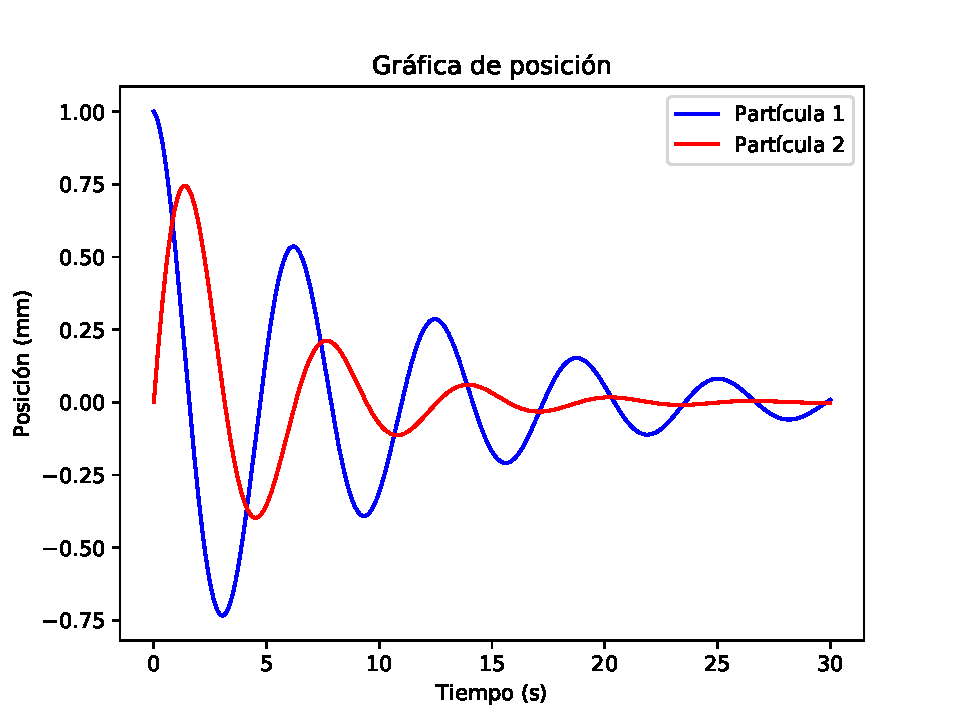
\includegraphics[width=0.55\textwidth]{img/ch03/plot_xlabel_ylabel_title.pdf}
	\caption{}
	\label{fig:plot_xlabel_ylabel_title}
\end{figure}

\subsection{Anotaciones}

Con anotaciones nos referimos a cualesquiera texto que se coloque dentro del \textit{Axes} de Matplotlib. Usualmente 
utilizadas para indicar ciertas características partículares en una gráfica, o bien alguna nota informativa al respecto.
La función base para realizar este tipo de tareas es \code{text}. La sintaxis más simple de \code{text} es:

\begin{python}
plt.text(px, py, texto)
\end{python}

Donde \code{px} y \code{py} denotan las coordenadas en donde se colocará la anotación indicado en \code{texto}. 
Veamos un ejemplo:

\begin{python}
import matplotlib.pyplot as plt
import numpy as np

x = np.linspace(0, 30, 200)
y = np.exp(-0.1*x)*np.cos(x)
plt.plot(x, y, "m")
plt.xlabel("Tiempo (s)")
plt.ylabel("Posición (mm)")
plt.title("Gráfica de posición")
plt.text(10, 0.5, "Algo informativo")
plt.show()
\end{python}

El código anterior produce la gráfica mostrada en la figura \ref{fig:plot_text}. Note que únicamente colocamos 
el texto \textit{Algo informativo}  dentro del gráfico, de manera más específica en las coordenadas (10,0.5).

\begin{figure}[H]
	\centering
	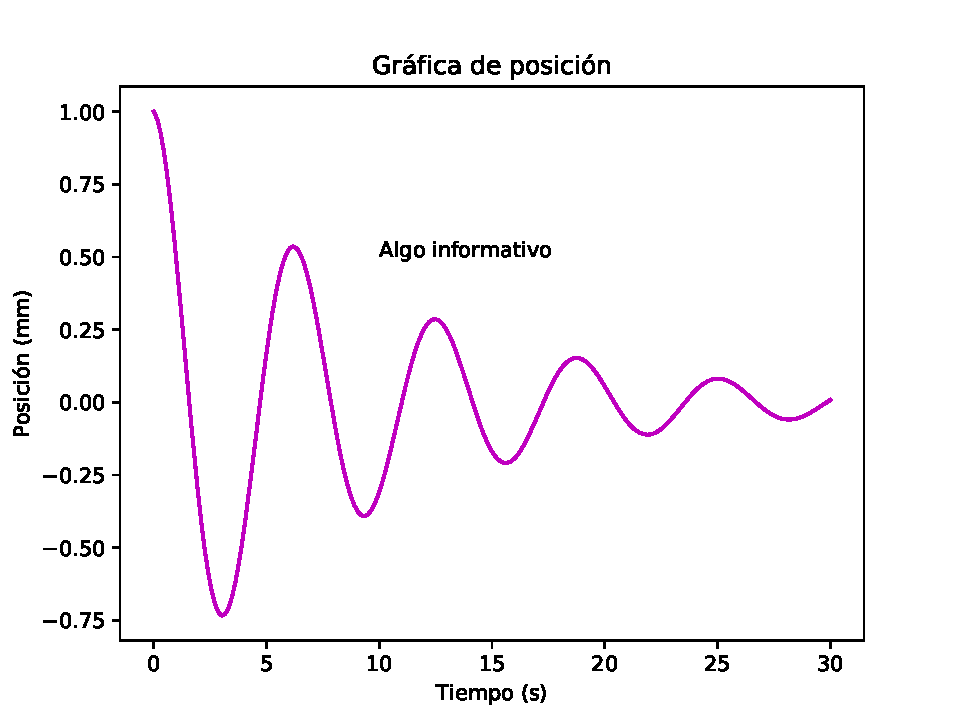
\includegraphics[width=0.55\textwidth]{img/ch03/plot_text.pdf}
	\caption{}
	\label{fig:plot_text}
\end{figure}

Al texto colocado podemos darle formato y ajustarlo a nuestros requerimientos, para ello a la función 
\code{text} se le pueden incluir los \textit{keyword arguments} descritos en \link{https://matplotlib.org/users/text_props.html}. 
Por ejemplo:

\begin{python}
import matplotlib.pyplot as plt
import numpy as np

x = np.linspace(0, 30, 200)
y = np.exp(-0.1*x)*np.cos(x)
plt.plot(x, y, "m")
plt.xlabel("Tiempo (s)")
plt.ylabel("Posición (mm)")
plt.title("Gráfica de posición")
plt.text(10, 0.5, "Algo informativo", fontsize=16, color="r", 
         name="Courier New")
plt.show()
\end{python}

Este código produce la gráfica mostrada en \ref{fig:plot_text_2}, observe que lo único que se cambió fueron algunas 
propiedades del texto, tales como el tamaño de la fuente con \code{fontsize}, el color de fuente con \code{color} 
y el tipo de fuente con \code{name}, con este último se debe tener cuidado, dado que el nombre de la fuente indicada 
debe estar instalada en la PC que se ejecuta. 

\begin{figure}[H]
	\centering
	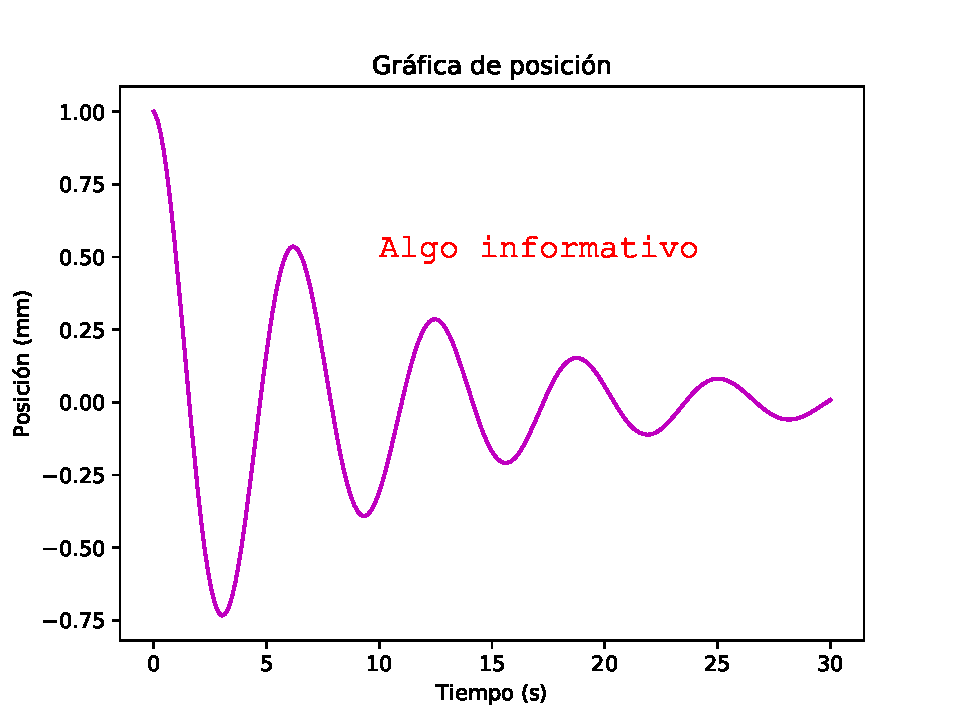
\includegraphics[width=0.55\textwidth]{img/ch03/plot_text_2.pdf}
	\caption{}
	\label{fig:plot_text_2}
\end{figure}


\section{Gráficas en coordenadas polares}

Las coordenadas polares o sistema de coordenadas polares son un sistema de coordenadas bidimensional en el que cada punto del plano se determina por una distancia y un ángulo \footnote{Tomado de: https://es.wikipedia.org/wiki/Coordenadas\_polares}. Habitualmente 
las funciones en coordenadas polares tienen la forma $ r = f(\theta)$.

En Matplotlib se dispone de la función \code{polar}, la cual traza una gráfica en coordenadas polares, dados como argumentos 
tanto la variable independiente $\theta$ como la función $r$. Enseguida vamos a ver cómo graficar la tan conocida 
\textbf{rosa polar}, cuya ecuación general está dada por:

$$ r = a \cos\left( k\theta + \phi_0 \right) $$

Implementando esto en Python, se tiene:

\begin{python}
import matplotlib.pyplot as plt
import numpy as np

theta = np.linspace(0, 2*np.pi, 1000)
a,k,phi0 = 5,7,0
r = a*np.cos(k*theta + phi0)
plt.polar(theta, r, "r")
plt.show()
\end{python}

El código anterior produce la gráfica mostrada en \ref{fig:polar_01}. Observe que la función \code{polar} 
funciona de manera bastante similar a \code{plot}, de hecho se le pueden pasar los mismos 
\textit{keyword arguments} para personalizar el gráfico resultante.

\begin{figure}[H]
	\centering
	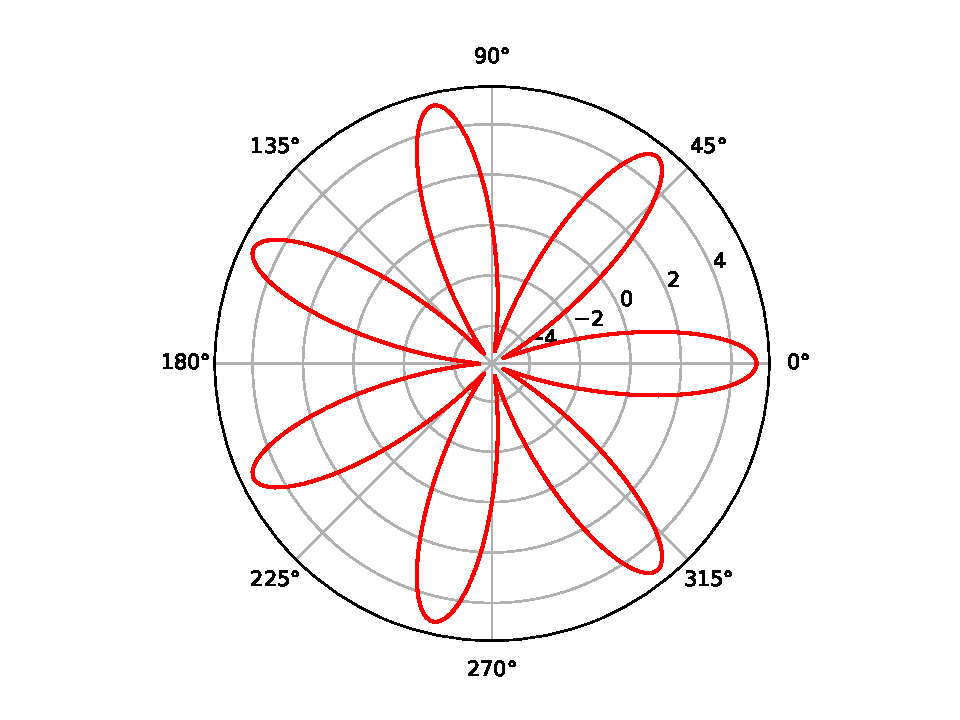
\includegraphics[width=0.55\textwidth]{img/ch03/polar_01.pdf}
	\caption{}
	\label{fig:polar_01}
\end{figure}


\section{Gráficas de barras}



\section{Gráficas de curvas paramétricas en el espacio}

Una función vectorial de la forma: 

$$ \vec{r}(t) = \begin{bmatrix}
x(t) \\ y(t) \\ z(t)
\end{bmatrix} $$

Se dice que es una función parámetrica, siendo $t$ en este caso el parámetro correspondiente. Una función vectorial 
de este tipo tiene una curva en el espacio asociada como representación gráfica. Es muy común 
trabajar con este tipo de expresiones en el análisis cinemático de partículas.

Supongamos que queremos graficar la función vectorial:

$$ \vec{r}(t) = \begin{bmatrix}
\cos(t) \\ \sin(t) \\ t	
\end{bmatrix} $$

En el intervalo $ 0 \leq t \leq 4\pi $. Para ello en Python haríamos lo siguiente:

\begin{python}
from mpl_toolkits.mplot3d import Axes3D
import matplotlib.pyplot as plt
import numpy as np

fig = plt.figure()
ax = fig.add_subplot(111, projection="3d")

t = np.linspace(0, 4*np.pi, 100)
x = np.cos(t)
y = np.sin(t)
z = t

ax.plot(x, y, z)
plt.show()
\end{python}

En la figura \ref{fig:parametric_curve_01} se muestra la gráfica producida. Ahora explicamos lo referente al código 
anterior. Observe que en la primera línea importamos la clase \code{Axes3D} del módulo \code{mpl\_toolkits.maplot3d}, 
esto nos sirve para poder trabajar con gráficas tridimensionales. Luego, definimos un objeto de la 
clase \code{Figure} y lo asignamos a la variable \code{fig}, al objeto \code{fig} le añadimos un 
\textit{Axes} mediante el método \code{add\_subplot}, indicando que dicho \textit{axes} se utilizarán las 
proyecciones espaciales mediante el \textit{keyword argument} \code{projection}. Las siguientes cuatro líneas 
definen las ecuaciones parámetricas. Y, finalmente con el método \code{plot} del objeto \code{ax} trazamos la 
gráfica de la curva tridimensional, note que en este caso el método \code{plot}, recibe al menos tres argumentos: 
las coordenadas en x, y, z.

\begin{figure}[H]
\begin{subfigure}{0.48\textwidth}
\centering
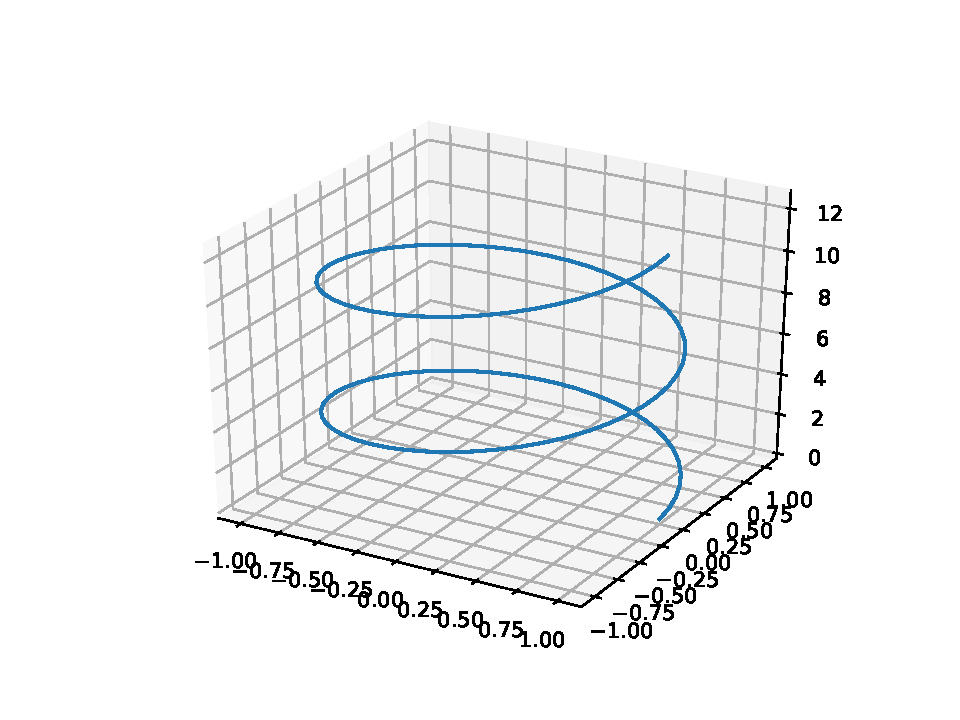
\includegraphics[width=0.9\textwidth]{img/ch03/parametric_curve_01.pdf}
\captionof{figure}{}
\label{fig:parametric_curve_01}
\end{subfigure}~
\begin{subfigure}{0.48\textwidth}
\centering
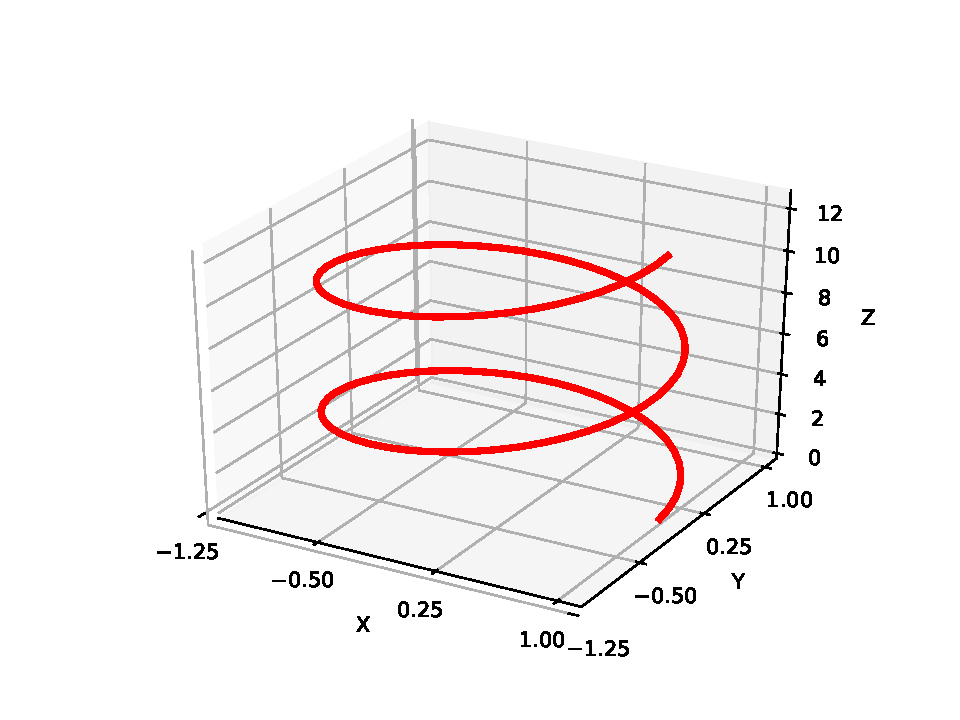
\includegraphics[width=0.9\textwidth]{img/ch03/parametric_curve_02.pdf}
\captionof{figure}{}
\label{fig:parametric_curve_02}
\end{subfigure}

\caption{}
\end{figure}

Al igual que en las otros tipos de gráficos, podemos también manipular las características. Vea por 
ejemplo el siguiente código:

\begin{python}
from mpl_toolkits.mplot3d import Axes3D
import matplotlib.pyplot as plt
import numpy as np

fig = plt.figure()
ax = fig.add_subplot(111, projection="3d")

t = np.linspace(0, 4*np.pi, 100)
x = np.cos(t)
y = np.sin(t)
z = t

ax.plot(x, y, z, color="r", linewidth=3)
xticks = ax.get_xticks()
yticks = ax.get_yticks()
ax.set_xticks(xticks[::3])
ax.set_yticks(yticks[::3])
ax.set_xlabel("X")
ax.set_ylabel("Y")
ax.set_zlabel("Z")
plt.show()
\end{python}

La gráfica producida se muestra en la figura \ref{fig:parametric_curve_02}.


\section{Gráficas de superficies}


\section{Ejercicios}

\begin{enumerate}
\item Grafique las siguientes funciones en el intervalo indicado:
\begin{enumerate}
\item $ y = \cos x + x \qquad 0 \leq x \leq 6\pi $ 
\item $ x = t^2 - 3t \qquad -10 \leq t \leq 10 $ 
\end{enumerate}

\end{enumerate}